\documentclass{article}
\usepackage[utf8]{inputenc}
\usepackage{authblk}

\title{Software engineering 2}
\author[1]{Saman Fekri}
\author[2]{Parniya Saeedzadeh}
\date{November 2020}

\usepackage{natbib}
\usepackage{graphicx}

\usepackage[table,xcdraw]{xcolor}
\definecolor{tableBorderColor}{rgb}{.58,.66,.84}
\definecolor{tableHighlightColor}{rgb}{.85,.89,.95}

\usepackage{tabularx}
\usepackage{longtable}

\usepackage{float} 

\usepackage{caption}
\captionsetup[figure]{labelfont={bf},labelformat={default},labelsep=period,name={Figure}, font={scriptsize,it}}

\usepackage[a4paper,bindingoffset=0.2in,%
            left=1in,right=1in,top=1in,bottom=1in,%
            footskip=.25in]{geometry}

\begin{document}

% \maketitle

% \section{Introduction}
% There is a theory which states that if ever anyone discovers exactly what the Universe is for and why it is here, it will instantly disappear and be replaced by something even more bizarre and inexplicable.
% There is another theory which states that this has already happened.\\
% ccadcdc 
% \begin{figure}[h!]
% \centering
% 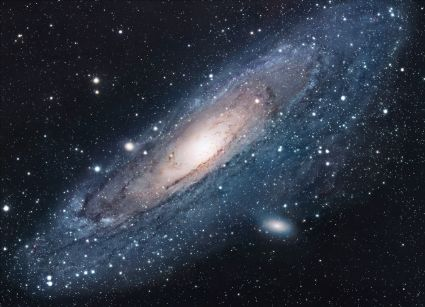
\includegraphics[scale=1.7]{universe}
% \caption{The Universe}
% \label{fig:universe}
% \end{figure}

% \section{Conclusion}
% ``I always thought something was fundamentally wrong with the universe'' \citep{adams1995hitchhiker}
% 
% \bibliographystyle{plain}
% \bibliography{references}

\section{First Part}
is here
\subsection{Instantaneous Velocity}

\subsection{Defining Instantaneous Velocity Using the Idea of a Limit}
\vfill
\section{Introduction}
\subsection{Purpose}
\paragraph{}
This document focuses on Requirements Analysis and Specification Document (RASD) and contains the description of the main goals, the domain and its representation through some models, the analysis of the scenario with the uses cases that describe them, the list of the most important requirements and specifications that characterize the development of the software described below.

\paragraph{}
It also includes the research about the interfaces, functional and non-functional requirements and the attributes that distinguish the quality of the system.

\paragraph{}
This document has the purpose to guide the developer in the realization of the software called CLup, a Customers Line-up application.

\paragraph{}
Finally, to understand better the development of the document, it contains the history that describes how it is made, with the references used and the description of its structure.

% table 
\begin{table}[hbt!]
\begin{tabular}{ l | l}
\hline
    \textbf{G1} & 2 \\  \hline
    \rowcolor[HTML]{34CDF9} salam & hi \\
    khobi & merCmerCmerCmerCmerCmerCmerCmerC \\ \hline
\end{tabular}
\end{table}

\subsection{Scope}
\subsection{Definition, Acronyms, Abbreviations}
\subsection{Revision history}
\subsection{Reference Documents}
\subsection{Document Structure}
\vfill

\section{Overal Description}

\subsection{Product perspective}
\subsubsection{UML Description}
The UML below describes at high-level the model of the system to be developed. It considers the basic service together with the advanced function 1 and advanced function 2 previously specified. The UML does not include every class that will be necessary to define the complete architecture of the system.\\
CLup more functions than basic service. The manager registers to the application with all necessary information and the manager could activate the advance function or advance function 2 at any time. The user who use mobile could simply download the application on his/her device and use it and user who doesn't have mobile could easily go near the shop and get a ticket from ticket machine.\\
Here we can identify the main aspect of CLup:
\begin{itemize}
    \item The user could request to be in line for a shop and application shows estimated waiting time to him/her.
    \item The user could book a visit for a shop. This booking contains the date and time user wants to go shopping besides, user can add the categories of item he/she has in shopping list. The application could suggest the user free slots and user book them.
    \item The application based the current location of users must notify them and ask them to approach the shop in a suitable time.
    \item The application must notify people when it's their turn to go shopping.
    \item At the entrance time, the QR code generated in the app must be scanned to ensure they come in the right time.
    \item At the checkout, the cashier must scan the QR code of user and the system must add shopping information (like duration of shopping, category of item which user buy) to user history.
\end{itemize}

\begin{figure}[H]
  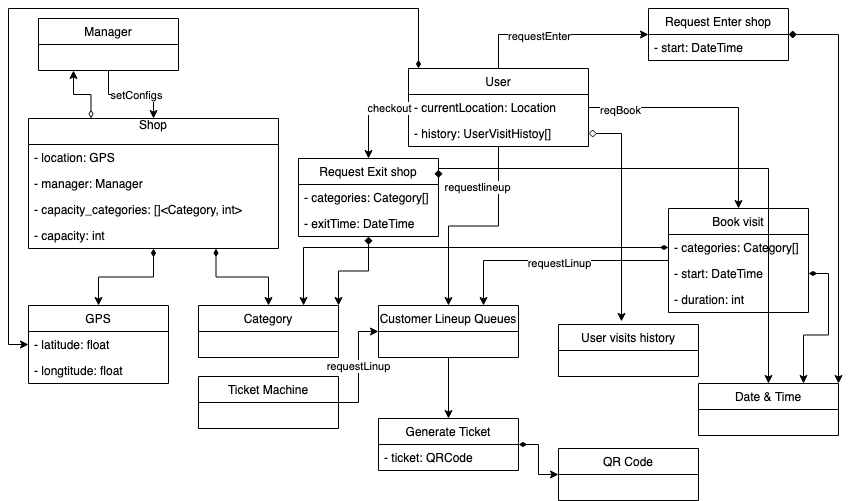
\includegraphics[width=\textwidth,height=\textheight,keepaspectratio]{images/ClassDiagram.png}
  \caption{High level Class Diagram}
  \label{fig:ClassDiagram}
\end{figure}

\subsubsection{State Diagrams}
Now we analyse the some important functions of the application, modelling their behaviours and analyze their behaviour to have the expected functionality. we report these diagrams below. \\

\begin{figure}[H]
  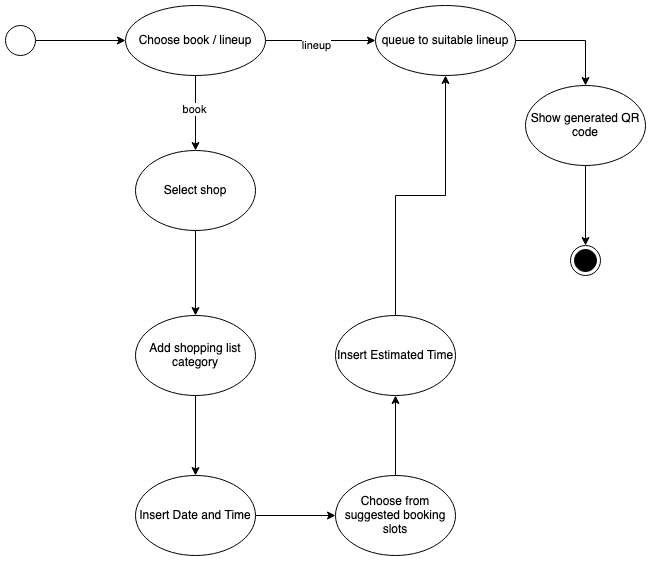
\includegraphics[width=\textwidth,height=\textheight,keepaspectratio]{images/bookLineup.png}
  \caption{User book a visit or insert to lineup queue}
  \label{fig:bookLineup}
\end{figure}

In this (Figure \ref{fig:bookLineup}), we model a user whom has a cell phone and wants to go shopping. As you can see, the user can choose to go to queue or book a visit for a time in future. System could sends him/her list of suggested time and user could choose between them.

\begin{figure}[H]
  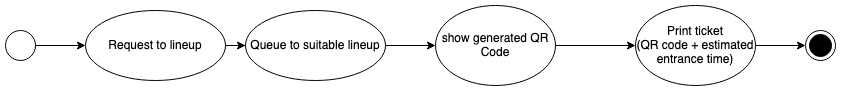
\includegraphics[width=\textwidth,height=\textheight,keepaspectratio]{images/OfflineTicket.png}
  \caption{User get ticket from ticket machine}
  \label{fig:OfflineTicket}
\end{figure}

In this (Figure \ref{fig:OfflineTicket}), we model a user who want to use ticket machine and do not use the app. In this case, user only can add himself/herself to the current line up of the shop.

\begin{figure}[H]
  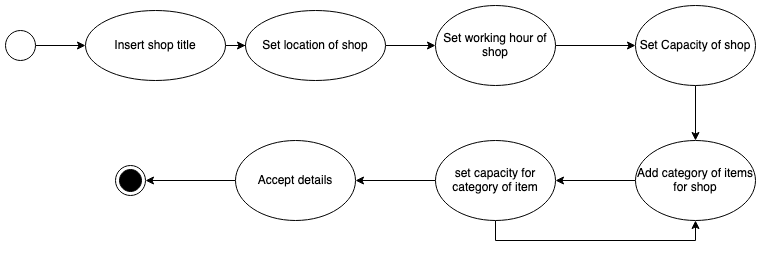
\includegraphics[width=\textwidth,height=\textheight,keepaspectratio]{images/CreateShop.png}
  \caption{Manager create a shop}
  \label{fig:CreateShop}
\end{figure}

In this (Figure \ref{fig:CreateShop}), shows how a manager could create a shop and add necessary information for creating a shop in our system.

\begin{figure}[H]
  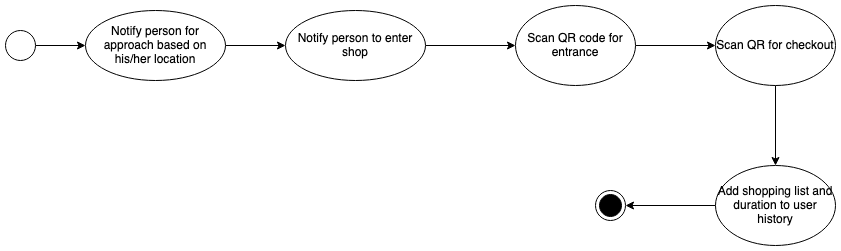
\includegraphics[width=\textwidth,height=\textheight,keepaspectratio]{images/Shopping.png}
  \caption{User shopping}
  \label{fig:shopping}
\end{figure}

In this (Figure \ref{fig:shopping}), we model the behaviour of user from entrance to shop until checkout. In the checkout time, we re-scan the QR code of user to insert data user shopping list and duration to user history. we could use, this information to estimate the behaviour of each user and improve waiting time estimation in our system.

\subsection{Product functions}
1. retrieving a number to line up: the main functionality of the application is the possibility of retrieving a number  which gives them their position in the queue. after then it will be easier for customers to access the supermarket without standing in a line for so long.  this way  forces people to first approach the building and then wait in close proximity (though not in a line) until their number is called.

2. generate QR codes:  this feature would be scanned upon entering the store, thus allowing store managers to monitor entrances.

3. estimation process:  There is a real risk that the approach does not
work in the case the customer arrives to the grocery store after his/her number is called, or too early, as in this case we would get back into a physical line situation. This implies that the system should provide customers with a reasonably precise estimation of the waiting time and should alert them taking into account the time they need to get to the shop from the place they currently are.

4. booking a visit: this function indicate that u can reserve a slot to go to supermarket, its almost like reserving a slot to go to museum or exhibition but they have slight differences like the duration that take to be in a supermarket which we are not able to estimate their time of shopping. so we have to mention a feature which request customer to indicate the approximate expected duration of the visit.

5. system for the customers analysis: there's another option that works for long-term customers in which the time spent by customers is analyzed and the system is gonna predict the average time for that specefic customer based on their pervious visits.

6. indicating the category of items: The application might also allow users to indicate, if not the exact list of items that they intend to
purchase, the categories of items that they intend to buy. This would allow the application to plan visits in a finer way, for example allowing more people in the store, if it knows that they are going to buy different things, hence they will occupy different spaces in the store when they visit (thus respecting the requirement that people keep enough distance between them).

\subsection{User characteristic}
The actors of the application are the following:

\begin{enumerate}
\item \textbf{user:} customers who download this application to go shopping for the groceries but due to Covid-19 stores and supermarkets shouldn't be full of people and they should follow the social distant rule so without application they used to stand in long lines with social distance but with this application which generate QR codes and with other functionalities, we minimize the time spent by each customer in a line by retrieving a number and send them to be in line if their number is getting closer. also they can book a visit from some days before to go for shopping at supermarkets.

\item \textbf{Clerk:} they would scan the QR codes which customers already have by app, and they allow customers to enter. Moreover, stores should also have the possibility to hand out “tickets” on the spot, thus acting as proxies for the customers because maybe some customers do not have the  access to the required technology

\item \textbf{Manager:} the manager is defining the store on our system and he/she assigns the capacity of either the whole store or each section of the that.
\end{enumerate}

\subsection{Assumptions, dependencies and constraints}
Domain assumptions: 
\arrayrulecolor{tableBorderColor}
\setlength\arrayrulewidth{1pt}
\rowcolors{2}{white}{tableHighlightColor}
\setlength\LTleft{0pt}

\begin{longtable}{ !\Vline c !\Vline p{0.9\linewidth} !\Vline}
    \hline
    \textbf{D1} & The internet works properly\\
    \textbf{D2} & Its better for users to have smartphones  \\
    \textbf{D3} & users should be at the spot right on the specific time which is mentioned in the app \\
    \textbf{D4} & the time estimation by the app is correct \\
    \textbf{D5} & Clerks are connected to device Which is registered for the specific shop.\\
     \textbf{D6} & the app is always available and able to generate QR codes\\
    \textbf{D7} & QR code on the ticket of each user must be scan first then let the user to enter the shop.\\
     \textbf{D8} & the QR code shown by users to scanner is valid\\
    \textbf{D9} & At the checkout, QR code on the ticket of each user must be scanned.\\
    \textbf{D10} & the slots shown by app is correct and updated every second for booking part\\
    \textbf{D11} & the QR code generator which called ticket machine for those who doesn't have smartphones works properly all the time\\
    \textbf{D12} & QR code scanner just scan the valid QR codes which means it shouldn't scan after the estimated time.\\
    \textbf{D13} & users do not have much delay at the supermarket and they exit at almost certain time.\\
    \textbf{D14} & Ticket machine should have enough paper to print QR codes for those who doesn't have smartphone.\\
    \textbf{D15} & if users don't have electronic device, they can use QR codes at the supermarket in person by ticket machine.\\
    
    \hline
\end{longtable}

Constraints:
\arrayrulecolor{tableBorderColor}
\setlength\arrayrulewidth{1pt}
\rowcolors{2}{white}{tableHighlightColor}
\setlength\LTleft{0pt}

\begin{longtable}{ !\Vline c !\Vline l !\Vline}
    \hline
    \textbf{C1} & each ticket is valid for entrance from time the system call it turns until 30 minutes later\\
    \hline
\end{longtable}


\end{document}
